\documentclass[11pt,a4paper]{article}

\usepackage[T1]{fontenc}
\usepackage[ngerman]{babel}
\usepackage[utf8]{inputenc}

\usepackage{amsmath}
% \usepackage{mathtools}

\usepackage[tt=false]{libertine}   % !!!!! das muss man nicht nutzen
\usepackage[libertine]{newtxmath}  % !!!!! das muss man nicht nutzen
%\usepackage[supstfm=libertinesups,supscaled=1.2,raised=-.13em]{superiors}
% params taken from doc

%
%\usepackage{tgpagella}
%\usepackage[euler-digits]{eulervm}
%
\usepackage{csquotes}

\usepackage{microtype}

\usepackage{fancyvrb}

\usepackage{graphicx}

\usepackage{booktabs}
\usepackage[shortlabels]{enumitem}
\setlist{noitemsep}

\usepackage{titlesec}
\usepackage{tcolorbox}
\tcbuselibrary{listingsutf8}

\usepackage{bbold}
\newcommand{\Z}{\mathbb{Z}}

\usepackage{hologo}

%-----------------------------------------------------------------------------
% für das Deckblatt

\usepackage{tikz}

\newcommand{\teilnehmername}{Klaus Philipp Theyssen} % !!!!!
\newcommand{\teilnehmermatrnr}{2061578}        % !!!!!
\newcommand{\seminarart}{Proseminar}           % !!!!!  oder Seminar
\newcommand{\seminarlp}{3 LP}                  % !!!!!  Prosem: immer 3 LP, 
\newcommand{\seminarjahr}{2019}                % !!!!!
%-----------------------------------------------------------------------------
\newcommand{\meta}[1]{$\langle$\textit{#1}$\rangle$}
\newcommand{\paket}[1]{\texttt{#1}}
\newcommand{\prgname}[1]{\texttt{#1}}

%-----------------------------------------------------------------------------
\author{Klaus Philipp Theyssen}
\title{Proseminar Ausarbeitung Brown'sche Schaltkreise}

%=============================================================================
\begin{document}
%=======================================================================
% Anfang erste Seite
{\thispagestyle{empty}\large\sffamily\raggedright
%
\begin{tikzpicture}[remember picture,overlay]
  \coordinate[xshift=5mm,yshift=-5mm] (NW) at (current page.north west) {};
  \coordinate[xshift=-5mm,yshift=-5mm] (NE) at (current page.north east) {};
  \coordinate[xshift=-5mm,yshift=13mm] (SE) at (current page.south east) {};
  \coordinate[xshift=5mm,yshift=13mm] (SW) at (current page.south west) {};

  \draw[line width=0.25pt] (NW)
    [rounded corners=5mm] -- (NE) 
    [sharp corners] -- (SE)
    [rounded corners=5mm] -- (SW)
    [sharp corners] -- cycle
  ;
\end{tikzpicture}
%
\unskip % keine Ahnung warum das nötig ist
\noindent \textbf{\Large \seminarart\ (\seminarlp)} 
\\[\baselineskip]
%
Zellularautomaten und diskrete komplexe Systeme
% für Fortgeschrittene  % nur für das 4 Leistungspunkte Seminar !!!!!
\\[1ex]
%
im Sommersemester \seminarjahr

\vspace*{3\baselineskip}

\noindent \textbf{\Large Ausarbeitung} \\[\baselineskip]
%
von \textbf{\teilnehmername}, Matr.nr.~\teilnehmermatrnr

\vspace*{3\baselineskip}

\noindent \textbf{\Large Thema} \\[\baselineskip]
%
% nachfolgend ein Beispiel, für Konferenzbeiträge, Buchausschnitte, ...
% bitte analog vorgehen !!!!!
%
 Ferdinand Peper and Jia Lee (2018)\\[1ex]
%
\textit{On Non-polar Token-Pass Brownian Circuits}\\[1ex]
%
Reversibility and Universality, S.299-311
}
\clearpage
% Ende erste Seite
%=======================================================================
% Anfang zweite Seite
{\thispagestyle{empty}\raggedright

\noindent \textbf{\Large Erklärung}\\[1ex]
gemäß \S 6 (11) der Prüfungsordnung Informatik % !!!!! oder \S 6 (7) 
(Bachelor) 2015 % oder Master !!!!!
\\[\baselineskip]

\noindent
Ich versichere wahrheitsgemäß, die Seminarausarbeitung zum
\seminarart{} "`Zellularautomaten und diskrete komplexe Systeme"' im
Sommersemester \seminarjahr{} selbstständig angefertigt, alle
benutzten Hilfsmittel vollständig und genau angegeben und alles
kenntlich gemacht zu haben, was aus Arbeiten anderer unverändert oder
mit Abänderungen entnommen wurde.

\vspace*{30mm}
\noindent
\begin{tabular}{@{}l}
  \hline
   \\[-1ex]
  \hbox to 0.6\textwidth{(\teilnehmername, Matr.nr.~\teilnehmermatrnr) \hss}
\end{tabular}
}
\clearpage
% Ende zweite Seite
%=======================================================================
%TODO Bilder mit verweisen und zitate mit verweisen
%TODO Rechtschreibung

%-----------------------------------------------------------------------------
\section{Einführung}
Bei Elektronik im nanometer Bereich sind Rauschen und Fluktuation 
entscheidende Faktoren die beim Entwurf entsprechender Schaltkreise 
zu beachten sind.
%
Desweitern ist ein geringerer Energieverbrauch anzustreben, daher 
werden in Zukunft Geräte von Interesse sein die nur von einzelnen 
Partikeln geschaltet werden.
%
Die in diesem Paper präsentiereten Brown'schen Schaltkreise nutzen Tokens
als Signale und setzen Fluktuation aktiv bei ihren Berechnungen ein.
Die Fluktuation orientiert sich dabei an der Brown'schen Molekularbewegung 
in der Biologie.
%
In \cite{Peper_Fundamentals_2013} wurden Brown'sche Schaltkreise 
vorgestellt und das T-Element, welches für die Klasse von Schaltkreisen 
universell ist, eingeführt.



%-------------------------------------------------------------------------------
\section{Grundlagen}
Tokens sind diskrete nicht teilbare Einheiten die Signale modellieren.
%
Zunächst werden die im Paper behandelten Schaltkreis Typen vorgestellt 
um Unterschiede in Funktionalität und Aufbau hervorzuheben. 
%
Dann wird das T-Element betrachtet und wie sich damit die Universaltät der
Brown'schen Token pass Schaltkreise ergibt.
%
Allgemein sind alle hier vorgestellten Schaltkreise asynchron,
dies bedeutet sie haben keinen Zeitgeber und es kann nebenläufig zu 
Änderungen am Signal kommen.
%
Sie sind robust gegen Verzögerungen (delay-insentive),
was heißt das Verzögerungen in der Signalweiterleitung 
nicht zu unkorrekten Berechnungen führen.


\subsection{Token-based Schaltkreise}
Token basierte Schaltkreise sind wichtig für physikalische Implementierungen
bei denen Signale diskret sind.
%
Dabei basieren die Schaltungen auf der Bewegung
von einzelnen Ladungen. 
%
Ein Beispiel für token basierte Schaltkreise sind Petrinetze. 
%
Token basierte Schaltkreise die delay insentive sind können mit 
einer Menge von Schaltkreisprimitiven konstruiert werden, genauso 
wie synchrone Schaltkreise aus NOT-Gattern und UND-Gattern.
%
Eine solche Menge nennt man dann universell und Abbildung \ref{fig:tokenBased} gibt 
dafür ein Beispiel.
%
Dabei führt Merge zwei Tokens zu einem zusammen.
% 
Fork macht aus einem Token zwei.
%
Tria fügt zwei Tokens zusammen und je nach eingabe Kabel kommt
die Ausgabe auf ein bestimmtes Kabel.
%
Wobei das Zusammenführen beim Tria nur funktioniert wenn zwei Tokens da sind,
also ein einzelnes Token wartet solange bis ein zweites kommt.
%
Diese Funktionalität in asynchronen Schaltkreisen entspricht dem Takt in
synchronen Schaltkreises und ist deshalb hervorzuheben.
%

\begin{figure}[h]
       \centering
       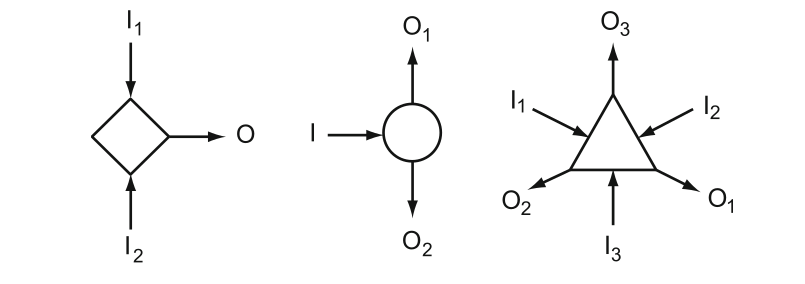
\includegraphics[width=9cm]{bilder/tokenBased.png}
       \caption{Merge, Fork und Tria}
       \label{fig:tokenBased}
\end{figure}    

%

\subsection{Brown'sche Schaltkreise}
Sie haben wie token-basierte Schaltkreise auch Tokens die sich auf Kabeln 
bewegen und in Schaltkreiselementen miteinander interagieren.
%
Allerdings wird hier die Interaktion durch Fluktuation getrieben und dient
als treibende Kraft für das Zusammenwirken der Tokens innerhalb der
Schaltkreiselemente. 
%
Dies ermöglicht Deadlocks mithilfe 
von Backtracking aufzulösen, was sich in einfacherem Design wiederspiegelt.


\subsection{Token-pass Schaltkreise}
Der Name kommt von der Bauweise dieser Schaltkreise, sie verbinden einfach nur
Kabel miteinander durch die Tokens hindurchlaufen.
%
Token-pass Schaltkreisen lassen die Zahl der Tokens gleich.
%
Tokens können nicht entstehen oder verschwinden und auch 
nicht auf andere Kabel wechseln.
%
Äquivalenz von Token-pass und token-based zeigen (ein kabel wird zu zwei)
die entsprechenden TP-Merge, TP-Fork, TP-Tria.
%
Token-pass Schaltkreise haben eine Menge an Eingabekablen die in
den Schaltkreis führen und eine Menge an Ausgabekabeln.
%
Dabei innerhalb des Schaltkreises können Schleifen sein. 
%

\begin{figure}[h]
    \centering
    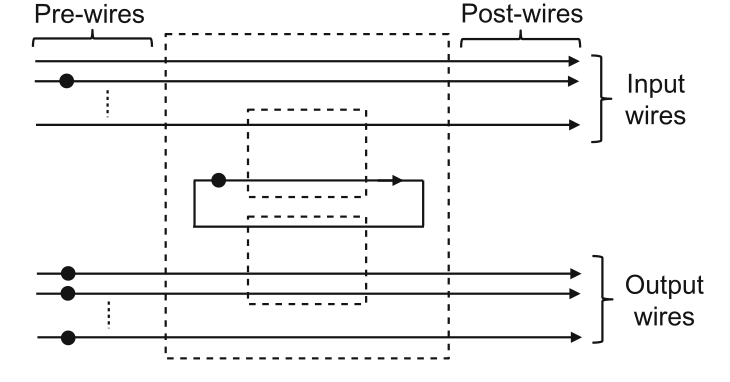
\includegraphics[width=8cm]{bilder/TokenPassScheme.png}
    \caption{Token Pass Schema}
    \label{fig:tokenPassScheme}
\end{figure} 

\subsubsection{Polare token-pass Schaltkreise}
In polaren token-pass Schaltkreises existiert eine bevorzugte Richtung
der Token, gekennzeichnet durch einen Pfeil.
%
Besonders bei den pre-Kabeln und post-Kabeln (also für Ein- und Ausgabe)
ist dies sinnvoll.

\subsubsection{Nicht polare token-pass Schaltkreise}
Hier können die Tokens frei fluktuieren, allerdings haben die T-Elemente eine
Einschränkung (kreise und blank symbole) wie sie Tokens verarbeiten.
%
Außerdem gibt es hier die möglichkeit von Terminatoren, dies sind Kabel
mit einem Ende auf dem Tokens sich einfach nur vor und zurück bewegen.
%
In einem nicht polaren token-pass Schaltkreis kann es aber auch vereinzelt
polare Kabel geben, wenn dies für die Berechnung Sinn macht.
%
Ein Beispiel sind die Ein- und AusgabeKabel da hier Tokens immer nur in eine 
Richtung gehen sollten und nicht nach erfolgreicher Berechnung diese 
wieder rückwärtslaufen.
%
Die nicht-polaren Schaltkreise ermöglichen einfacheres Design und Verwendung
von weniger T-Elementen, weil bestimmtes Verhalten zum Verhindern von
Deadlocks nicht expizit modelliert werden muss.

%-----------------------------------------------------------------------------
\section{T-Element}
Grundlegende Funktion des T-Elementes entspricht mit Abbildung 3.
%
Eingang c ist der Basis Eingang des T-Elmentes hier muss immer ein Token
anliegen damit es zur Verarbeitung kommt.
%
Wenn jetzt bei c ein Token anliegt und bei einem der beiden anderen
Eingänge a oder b noch ein Token anliegt werden diese vom T-Element 
entlang des gestrichelten Halbkreises auf das parallel verlaufende 
Kabel überführt.
%
Wenn bei a und b ein Token anliegt wird zufällig 
eines der beiden ausgewählt und mit c überführt.

\begin{figure}[h]
    \centering
    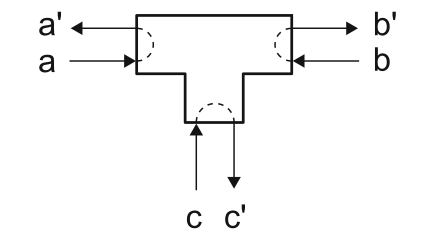
\includegraphics[width=7cm]{bilder/T_Element.png}
    \caption{T-Element}
    \label{fig:T_Element}
\end{figure}    

In Abbildung 4 ist zu erkennen wie die token basierten Schaltkreispirmitive 
(Merge, Fork und Tria) mit mithilfe des T-Elementes nachgebaut werden.
%
Theorem: Das brown'sche T-Element ist universell für die Klasse der token pass 
Schaltkreise.

\begin{figure}[h]
    \centering 
    \centering
    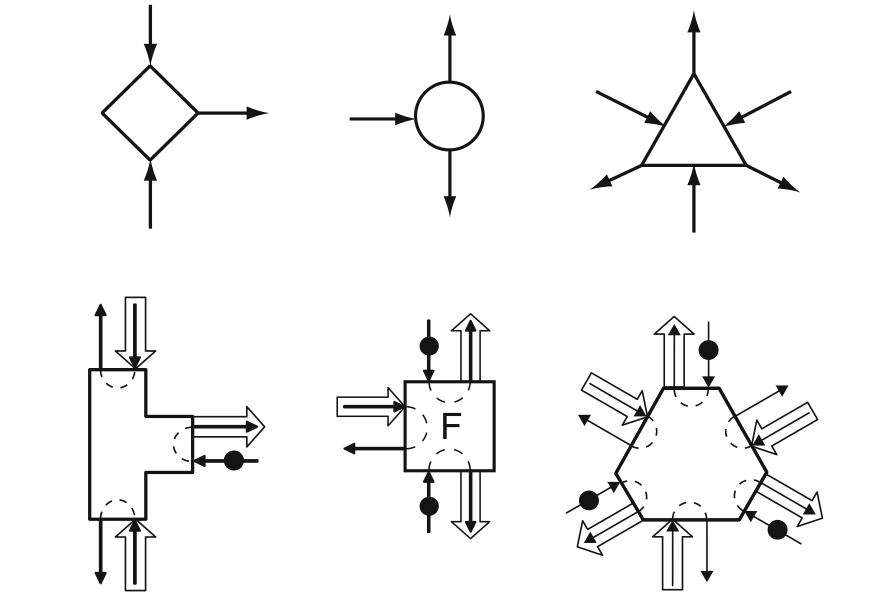
\includegraphics[width=7.5cm]{bilder/BasedToPass.png}
    \caption{Äquivalenz Token based Token pass}
    \label{fig:BasedToPass}
\end{figure}


\begin{figure}[h]
     \begin{minipage}{0.45\textwidth}
        \centering
        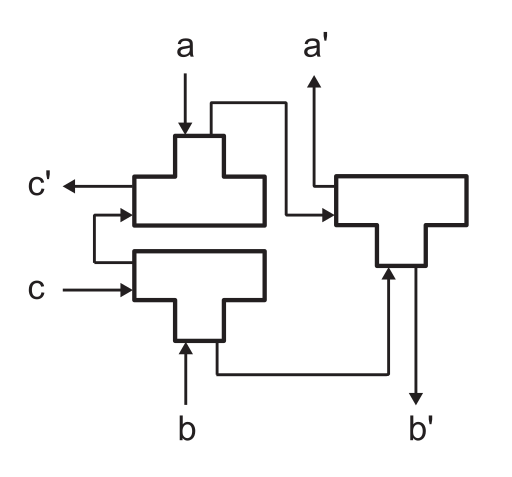
\includegraphics[width=6cm]{bilder/TP_Fork.png}
        \caption{Fork aus T-Elementen}
    \end{minipage}\hfill
     \begin{minipage}{0.45\textwidth}
        \centering
        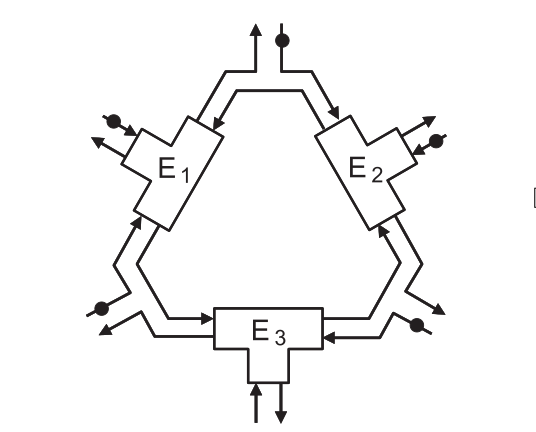
\includegraphics[width=6cm]{bilder/TP_Tria.png}
        \caption{Tria aus T-Elementen}
    \end{minipage}\hfill
\end{figure}    

%
Allerdings ist das Nachbauen von token basierten Schaltkreisen mithilfe
der TP-Merge, TP-Fork und TP-Tria nicht effizient.
%
Da hier die Besonderheit des Fluktuierens der Tokens nicht ausgenutzt wird.
%
Beispielsweise benötigt ein 1-Bit Speicher der naiv mithilfe der 
Schaltkreisprimitiven nachgebaut ist insgesamt 26 T-Elemente.
%
Im nächsten Abschnitt werden wir sehen das dies 
sehr viel effizienter möglich ist wenn man Eigenschaften der brown'schen 
token pass Schaltkreise beim Design richtig ausnutzt.

%-----------------------------------------------------------------------------
\section{1-Bit Speicher}
Nun soll anhand eines 1-Bit Speichers die Funktionsweise von brown'schen 
token-pass Schaltkreisen erläutert werden.
%
Mithilfe von polaren T-Elementen ist es möglich einen 1-Bit Speicher mit 8
T-Elementen zu bauen \cite{Peper_Fundamentals_2013}. 
%
Bei nicht-polaren brown'schen T-Elementen sind es sogar
nur 7 \cite{Peper_nonPolar_2018}.
%

\begin{figure}[h]
      \centering
      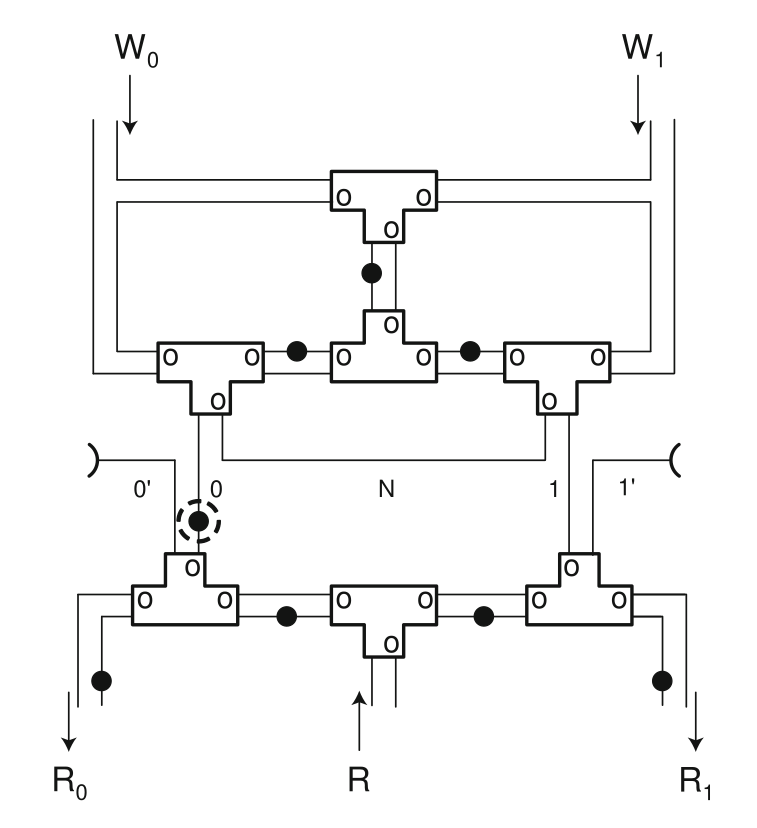
\includegraphics[width=9cm]{bilder/NonPolarMemory.png} 
      \caption{1-Bit Speicher nicht polar token pass}
\end{figure}

\subsection{Nicht polarer token-pass 1-Bit Speicher}
Es werden nur 7 T-Elemente benötigt auch, hier Konzept von Lesen und Schreiben
erklären und Bedeutung/ Nutzen von Terminator Kabeln.
Das Deadlock Backtracking zeigen.

%-----------------------------------------------------------------------------
\section{UND-Bauteil}

\begin{figure}[h]
    \centering
    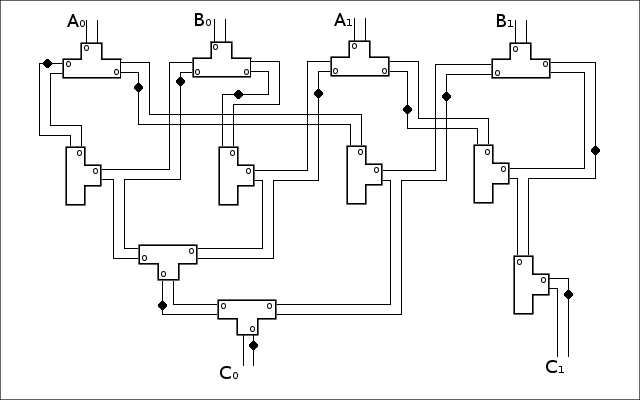
\includegraphics[width=12cm]{bilder/UndGatter.png}
    \caption{UND-Gatter aus 11 T-Elementen}
\end{figure}    

Als Teil meiner Eigenarbeit im Rahmen dieses Proseminars habe ich ein UND-Gatter
mithilfe von nicht-polaren T-Elementen entworfen.
%
Es benutzt den Deadlock Backtracking Mechanismus und jede 
mögliche Eingabe wird mit jeder möglichen Ausgabe und-verknüpft. 
%
Dabei werden zunächst T-Element zum modellieren der möglichen Wege benutzt,
die beiden Eingabe Token versuchen sich also zu entsprechend zu finden.
%
Haben sich beide Input Tokens gefunden wird ein Token weitergeleitet bei 
den Eingaben A1 und B1 wird dieses Token direkt zu Ausgabe C1, bei allen 
anderen Eingabemöglichkeiten werden die Token mithilfe von zwei weiteren 
T-Elementen zusammengeführt für die Ausgabe C0.


\subsection{Initialisierung}
Es ist eine Initialisierung auf der Abbildung gegeben (die Position der Tokens), 
außerdem sind die Kreise in den T-Elementen für eine korrekte Berechnung
elementar.
%
Diese Initialisierung ist nicht eindeutig und auch die Anordnung der
Elemente ist veränderbar, was im Hinblick auf möglichst kurze Kabel 
für eine schnellere Berechnung von Interesse ist.

\subsection{Korrektheit}
Eine interessante Frage ist nun ob die Korrektheit dieses Schaltkreises
beweisbar ist. Wenn wir die angegebene Initialisierung vorraussetzen können,
können wir uns die Korrektheit schnell klar machen indem :
%TODO mögliche Token interaktionen druchspielen OBdA für einen Fall



% ----------------------------------------------------------------------------
\section{Zusammenfassung und Ausblick}
In dem Paper \cite{Peper_nonPolar_2018} wird eine neue Art
von Schaltkreis vorgestellt der zukünfitig in der Nanoelektronik eingesetzt
werden könnte.
%
Aufbauend auf den polaren Brown'schen token pass Schaltkreisen aus 
\cite{Peper_Fundamentals_2013} werden nicht polare Kabel und T-Elemente 
eingeführt deren Token keinen Bias in ein Richtung haben. 
%
Dabei ist das Konzept von Brown'scher Bewegung der Signale (Tokens) 
der interessante und neue Aspekt der es ermöglicht neue Arten von Schaltkreisen 
zu designen und auf ihre Eigenschaften zu untersuchen.
%
Jedoch sind Dinge wie Geschwindigkeit der Berechnung, Korrektheit beweisen und 
welche arten von konkreten Implementierungen möglich sind noch zu klären.


\subsection{Geschwindigkeit der Berechnung}
Die Fluktoation der Tokens auf einem Kabel der Länge L führt zu 
erwartet Zeit 0(L²).
%
Desweiteren kann man Sperren einsetzen, sodass Tokens
auf bestimmten Kabeln sich nur in eine Richtung bewegen können. 
%
Dies ist auf den Ausgabekabeln sinnvoll.


\subsubsection{Ein langes Kabel vs. viele T-Elemente}
Eine interessante Frage wäre außerdem wie sich die Geschwindigkeit eines 
Token um eine gewisse Strecke zu überfinden verhält. 
%
Wenn einerseits nur ein langes Kabel durchlaufen wird. 
%
Oder meherere T-Elemente zwischengebaut sind bei denen das Token jeweils
am Basis Eingang ankommt um das Signal weiterzuleiten.
% 
Damit verbunden ist die Frage wann genau zwei Token vom T-Element 
verarbeitet werden, müssen diese in einem gewissen Bereich vorliegen (diskret).

\subsection{Design und Korrektheit}
Zwar sind mit nicht polaren brown'schen Schaltkreisen Schaltkreiselemente mit
weniger Bauteilen möglichen.
%
Allerdings ist das Vorgehen beim Entwerfen und Überprüfen dieser Art von 
Schaltkreisen auf Korrektheit noch unklar. 


\subsection{Implementierung}
Das T-Element ist geeignet um theoretisch dieses Berechnungsmodell zu 
untersuchen ist jedoch für eine Implementierung nicht optmial.
%
Es hat zu viele Kabel und ist zu komplex um sinnvoll als Schaltkreisprimitv
eingesetzt zu werden. 
%
Allerdings ist es für simplere Schaltkreiselemente nicht möglich in auch ohne 
Fluktuation zu funktionieren.
%
Auch kann es zu Interaktionen zwischen Tokens kommen die von bei diesem Modell
nicht beachtet werden. (z.B. Elektronen als Tokens und entsprechende 
Elektromagnetische Felder)
%
Auch kann es zu Interaktionen zwischen Tokens kommen die von bei diesem Modell
nicht beachtet werden. (z.B. Elektronen als Tokens und entsprechende 
Elektromagnetische Felder). Desweiteren sind Dinge wie Token bleiben nur
auf einem Kabel nicht unbedingt leicht um zu setzen für die Implementierung.



% Literaturverzeichnis erstellen 
\bibliographystyle{plain}
\bibliography{\jobname}

\end{document}
